

In the proposed architecture, the \textit{Smart Gateway} is the central module of the system, connecting the \textit{SmartBoxes} to the \acs{HIS}. It is responsible for the management of devices and their associations -- \textit{SmartBox} to \textit{Biosticker} and \textit{SmartBox} to user -- managing, maintaining and storing the data that is generated by these, as well as handling any communication to and from the \acs{HIS}. 


\paragraph{} Regarding the hardware platform used to implement the \textit{Smart Gateway}, in context of the \acs{WoW} project, we use the Intel NUC NUC8i7BEH\footnote{\url{https://ark.intel.com/content/www/br/pt/ark/products/126140/intel-nuc-kit-nuc8i7beh.html}}.

\begin{figure}[H]
    \centering
    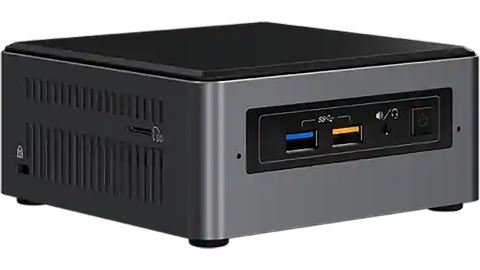
\includegraphics[width=0.4\linewidth]{images/gateway-image.png}
    \caption[Intel NUC NUC8i7BEH.]{Intel NUC NUC8i7BEH.}
    \label{fig:gateway_image}
\end{figure}


\paragraph{} In the next sections, we propose a service architecture for the \textit{Smart Gateway} in order to fulfill the aforementioned features.

% The \textit{Smart Gateway} maintains a list of all the \textit{SmartBoxes} that are managed by the system, as well as every \textit{Biosticker} and every sensor in the \textit{Biosticker} (which are used to indicate respective biosignal to the \acs{HIS}). 


\section{Service Architecture}

As we have seen, there are multiple key features that form the \textit{Smart Gateway}. From Figure \ref{fig:wow-architecture}, we can list the different \textit{Smart Gateway} components:  

\begin{itemize}
    \item \textbf{Manage devices and device associations}: The \textit{Smart Gateway} maintains a list of all the \textit{SmartBoxes} that are managed by the system, as well as every \textit{Biosticker} and every sensor in the \textit{Biosticker} (which are used to indicate the respective biosignal to the \acs{HIS}). The \textit{Smart Gateway} also tracks the sensor subscriptions per \textit{SmartBox}.
    \item \textbf{Data anonymization}: Any private data (\textit{i.e.} information that can be used to identify a user) that is stored in the \textit{Smart Gateway} is anonymized in order to meet data protection regulations\footnote{Resolution of the Council of Ministers no. 41/2018, of 28 March, following the new General Data Protection Regulation (GDPR), approved by Regulation (EU) 2016/679:  \url{https://dre.pt/application/file/a/114936962\%20}}. 
    \item \textbf{Data pre-processing}: The \textit{Smart Gateway} processes the data as it is collected in order to clean the data before storing it indefinitely, and to detect critical conditions of the patients' state to prompt an immediate notification to the health professionals.
    \item \textbf{Real-time data acquisition}: The \textit{Smart Gateway} acquires the data transmitted by \textit{SmartBoxes} in real-time. 
    \item \textbf{Manage data collection}: After receiving and processing the data from the \textit{SmartBoxes}, the \textit{Smart Gateway} stores indefinitely for long-term biomonitoring analytics.
    \item \textbf{\acs{HIS} \acs{FHIR} Integration}: The \textit{Smart Gateway} handles the communication with the \acs{HIS}, or more accurately, it processes \acs{FHIR} all requests from the \acs{HIS}, and also transforms the acquired sensor data into \acs{FHIR} messages and communicates it to the \acs{HIS}. 
\end{itemize}

To implement these components, we propose the following service architecture within the \textit{Smart Gateway}, as illustrated on Figure \ref{fig:gateway_serviceoverview}. The correspondence between the services and the \textit{Smart Gateway} components is described in Table \ref{tab:gateway-service}.

\begin{figure}[H]
    \centering
    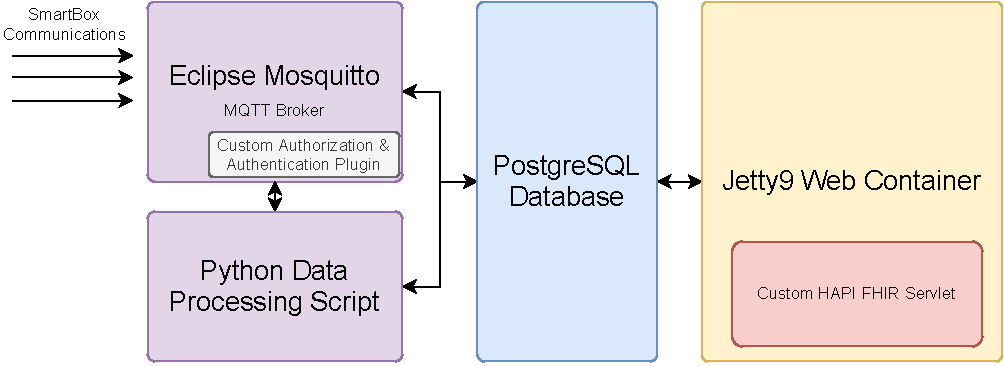
\includegraphics[width=0.8\linewidth]{images/service overview gateway.pdf}
    \caption[Service architecture implemented in the \textit{Smart Gateway}.]{Service architecture implemented in the \textit{Smart Gateway}. The diagram displays the different technologies used throughout the development. The services communicate with each other using Unix Domain Sockets, a Linux protocol for \acf{IPC}.}
    \label{fig:gateway_serviceoverview}
\end{figure}
\begin{table}[]
    \resizebox{\textwidth}{!}{%
    \begin{tabular}{ccc}
    \hline
    \textbf{Smart Gateway Module}          & \textbf{Smart Gateway Module} & \textbf{Description}                                                                                                                                                             \\ \hline
    Real-time data acquisition             & MQTT Broker                   & \makecell[c]{This service is responsible for \\ handling all smart boxes communication, ensuring data encryption, \\ authorization, etc.}                                                           \\
    Data pre-processing                    & Data processing               & \makecell[c]{This service is responsible for \\ data filtering and preliminary data processing.}                                                                                                  \\
    Manage data collection                 & \multirow{2}{*}{Data storage} & \multirow{2}{*}{\makecell[c]{This service holds and manages \\ critical system information, \\ such as authorized clients, permission \\ access for each client and \\ all of the collected sensor data.}} \\
    Manage devices and device associations &                               &                                                                                                                                                                                  \\
    Data anonymization                     & \multirow{2}{*}{FHIR Server}  & \multirow{2}{*}{This service is responsible for handling communications with  ``Interoperability'' layer  of \acs{HIS}.}                                                         \\
    \acs{HIS} \acs{FHIR} Integration       &                               &                                                                                                                                                                                 
    \end{tabular}
    }
\end{table}

\paragraph{} 

\subsection{Security on Linux}
%- o isolamento dos processos é feito através do "utilizador" que está a executar o processo, e é este o utilizador que delimita as permissões de e
- indicar que estamos a usar Unix Sockets para a comunicação entre processos \footnote{\url{https://man7.org/linux/man-pages/man7/unix.7.html}}; 

- o uso de unix sockets permite usar o sistema de permissões do sistema operativo para controlar o acesso às sockets (através dos ``utilizadores'' que estão a executar os serviços).

\paragraph{} As seen above, these services have 

\section{Data Storage}

The data storage in the \textit{Smart Gateway} is one of the most important components of the device, as it holds the information used by all services in the \textit{Smart Gateway}. Given the importance of this component, it is crucial to use a solution which offers reliability above all with great performance for our use case.  

\paragraph{} As discussed in Section \ref{sec:iot-model-layer4}, No\acs{SQL} databases are appealing for \acs{IoT} applications, since these have great performance..

% it is important to choose a solution which offers availability

% PostgreSQL offers a balance between \footnote{\url{https://itnext.io/benchmark-databases-in-docker-mysql-postgresql-sql-server-7b129368eed7?gi=a506815fb197}}

\subsection{Database Schema}
Figure \ref{fig:wow-dbschema-full} contains the database model implemented in our PostgreSQL database. It describes all information that is contained in the \textit{Smart Gateway}, the relations within that data, organized according to the functionality it is related to, which will be explored in greater detail in the next sections.

\begin{figure}[H]
    \centering
    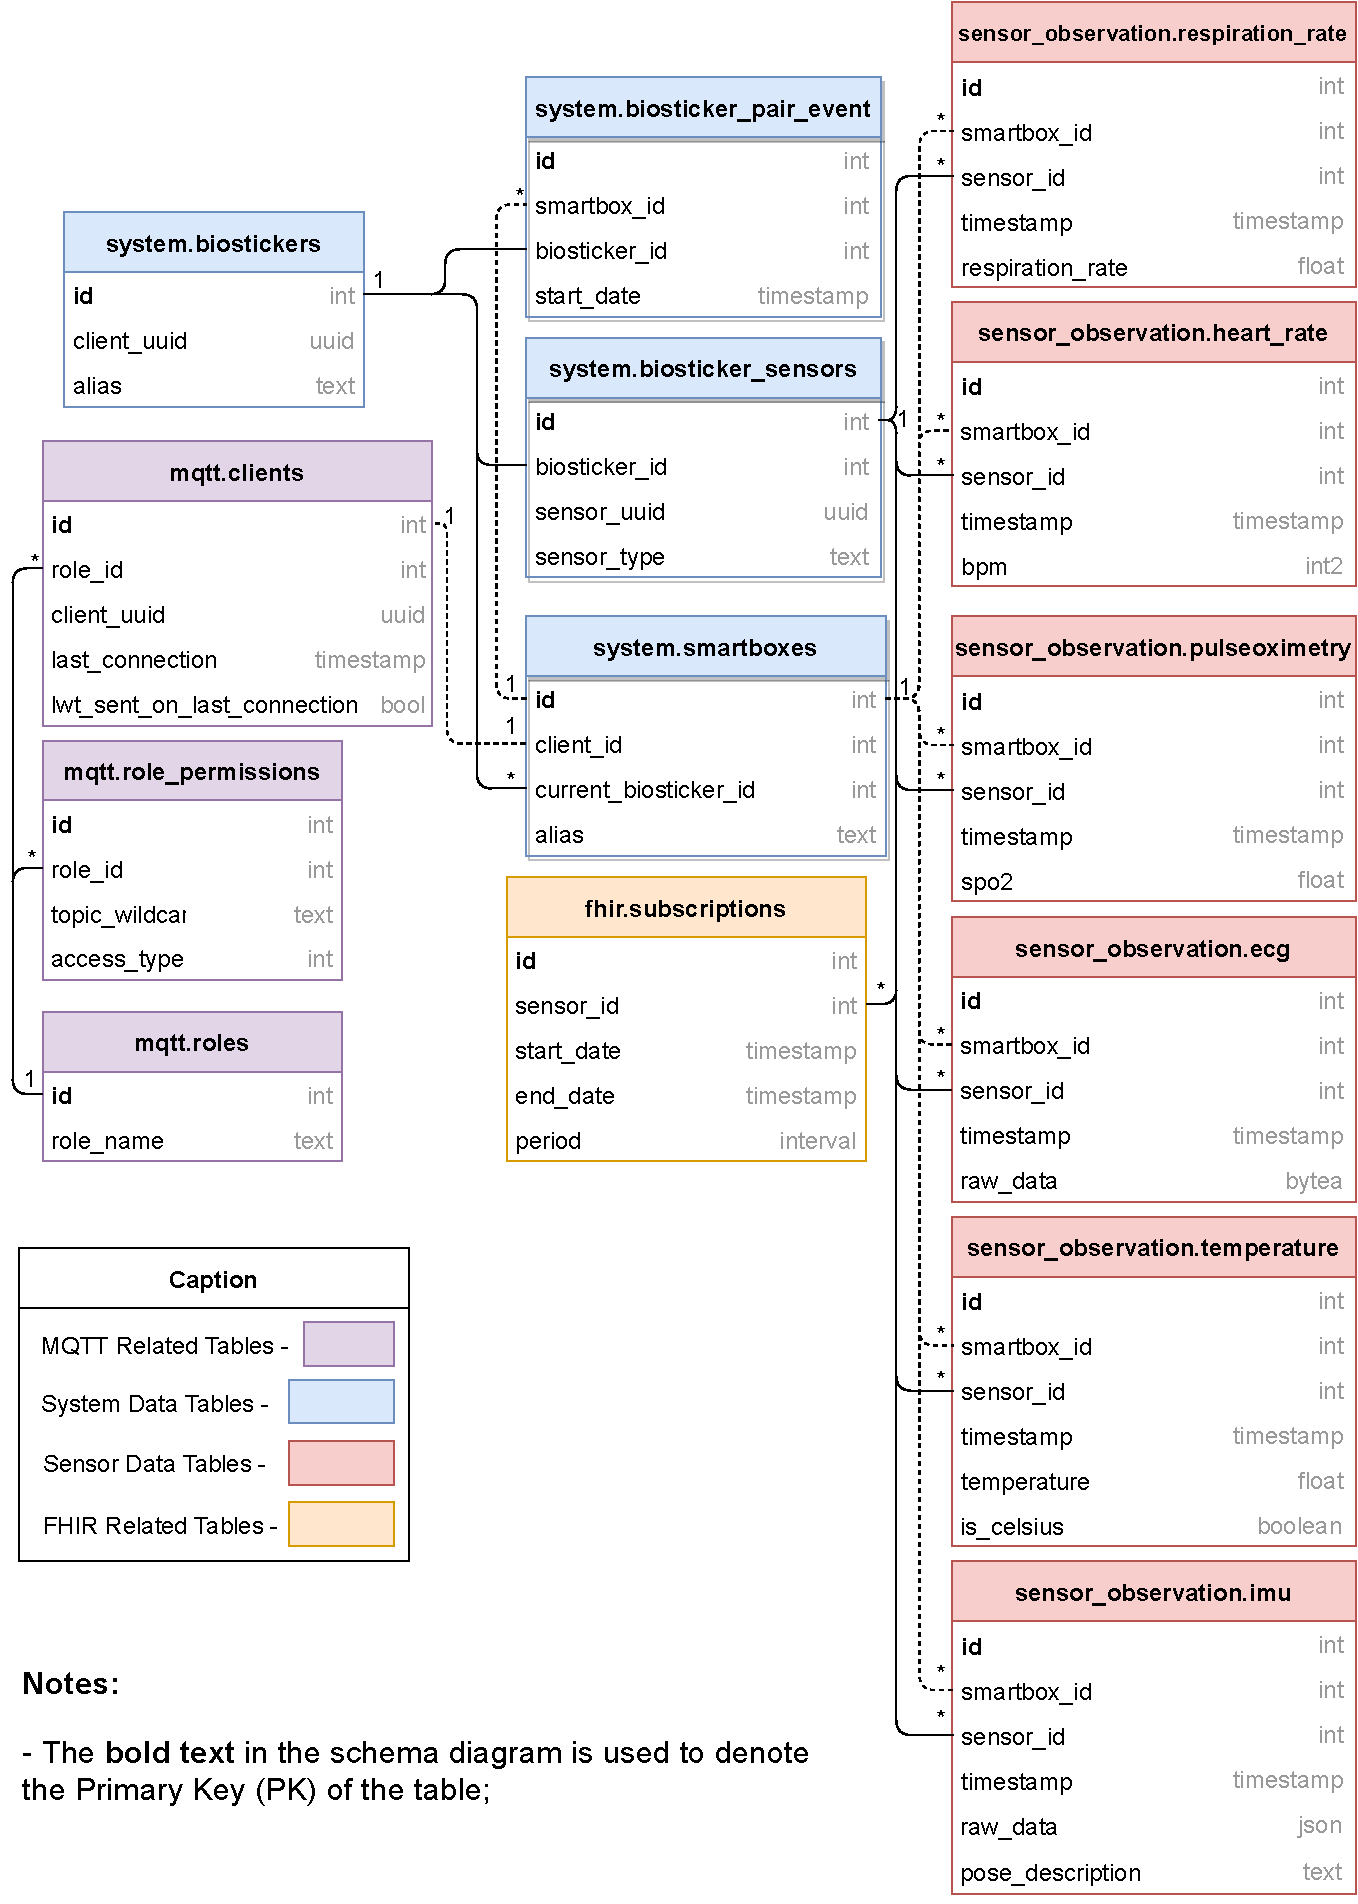
\includegraphics[width=0.86\linewidth]{images/database-schema-general.pdf}
    \caption[Database schema implemented in the \textit{Smart Gateway}.]{Database schema implemented in the \textit{Smart Gateway}.}
    \label{fig:wow-dbschema-full}
\end{figure}

\subsubsection{MQTT Client Information}

Figure \ref{fig:wow-dbschema-mqtt} contains the information relevant for \acs{MQTT} communications, mostly related with security. To ensure that each device only has access to its own resources, the system implements a \acf{RBAC} policy. 
In this type of access control, the system allows and revokes access to resources according to the role of the device. 

\paragraph{} In context of the \acs{WoW} project, the following roles are used:

\begin{itemize}
    \item \textit{SmartBox} role: Indicates the \acs{MQTT} client is a \textit{SmartBox}.
    \item ``Pyservice'' role: Indicates the \acs{MQTT} client is actually the data processing service, also contained in the \textit{Smart Gateway}.
    \item Developer device role: Indicates the \acs{MQTT} client is a developer device, used solely for debugging purposes.
\end{itemize}


\begin{figure}[H]
    \centering
    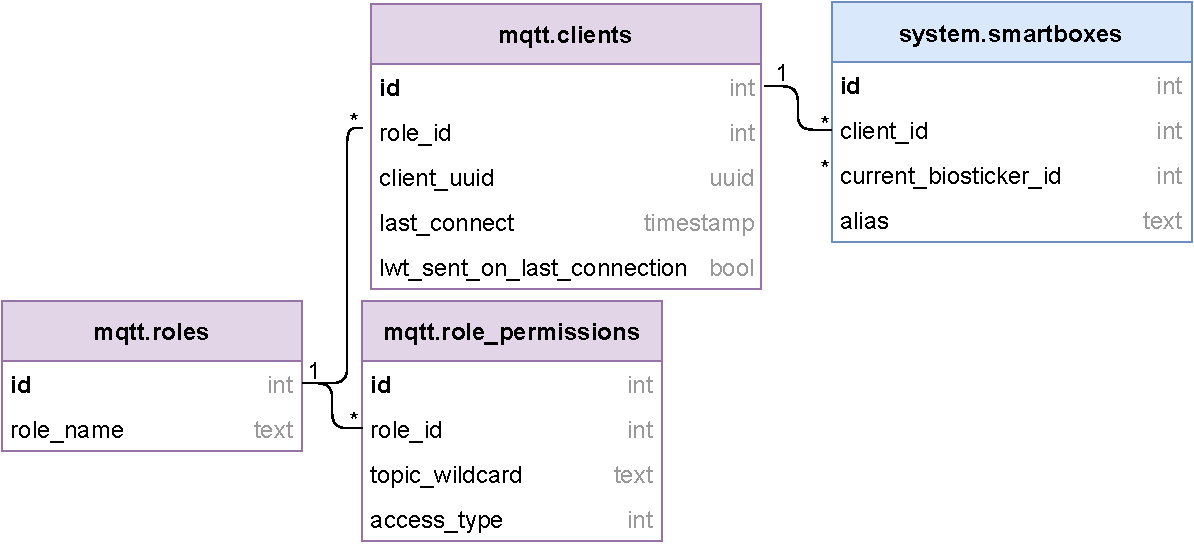
\includegraphics[width=\linewidth]{images/database-schema-mqtt.pdf}
    \caption[\acs{MQTT} information in the schema implemented in the \textit{Smart Gateway}.]{\acs{MQTT} information in the schema implemented in the \textit{Smart Gateway}.
    The ``mqtt.roles'' table contains the different \acs{RBAC} roles for the \acs{MQTT} communication and ``mqtt.role\_permissions'' table lists the permissions available to each role using \acs{MQTT} topic wildcards. The ``mqtt.client'' table lists the clients and their properties, such as their \acs{UUID}, the timestamp of their last connection, or a \textit{flag} to indicate if the communication failed during the last communication.
    
    }
    \label{fig:wow-dbschema-mqtt}
\end{figure}

\subsubsection{Sensor Data}

Figure \ref{fig:wow-dbschema-sensors} contains the sensor data collected over time. The tables 

\begin{figure}[H]
    \centering
    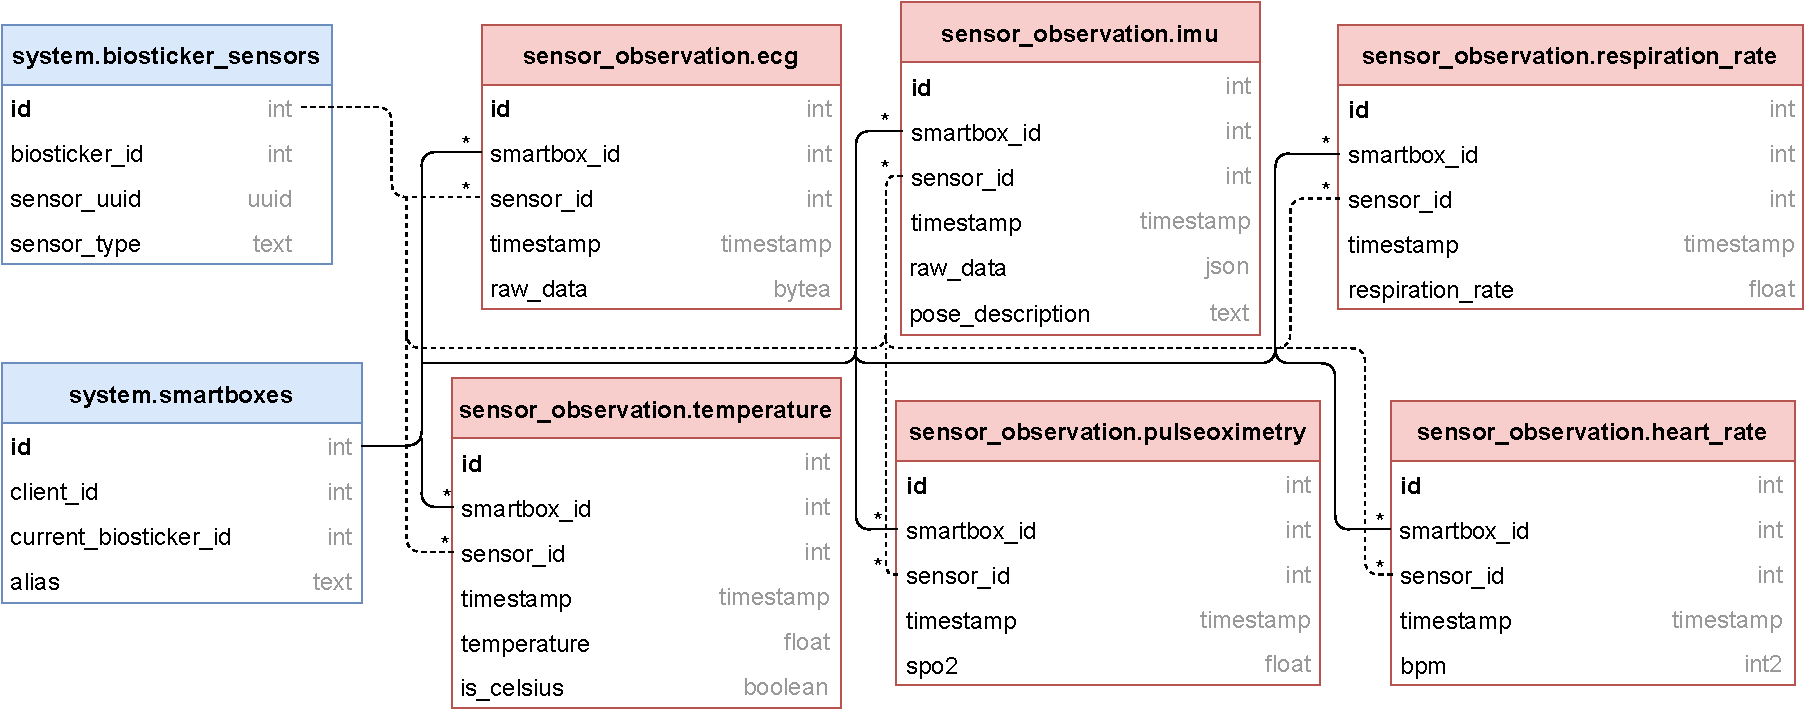
\includegraphics[width=\linewidth]{images/database-schema-sensordata.pdf}
    \caption[Sensor data information in the schema implemented in the \textit{Smart Gateway}.]{
        Sensor data information in the schema implemented in the \textit{Smart Gateway}. Our database model has one table for each different type of biosignal (temperature, \acs{ECG}, etc.). The properties of the table are defined according to the data acquired on the \textit{SmartBox} level, which are detailed in Section \ref{sec:biosticker_data}.}
    \label{fig:wow-dbschema-sensors}
\end{figure}

\subsubsection{FHIR Related Information}
\dots 

\begin{figure}[H]
    \centering
    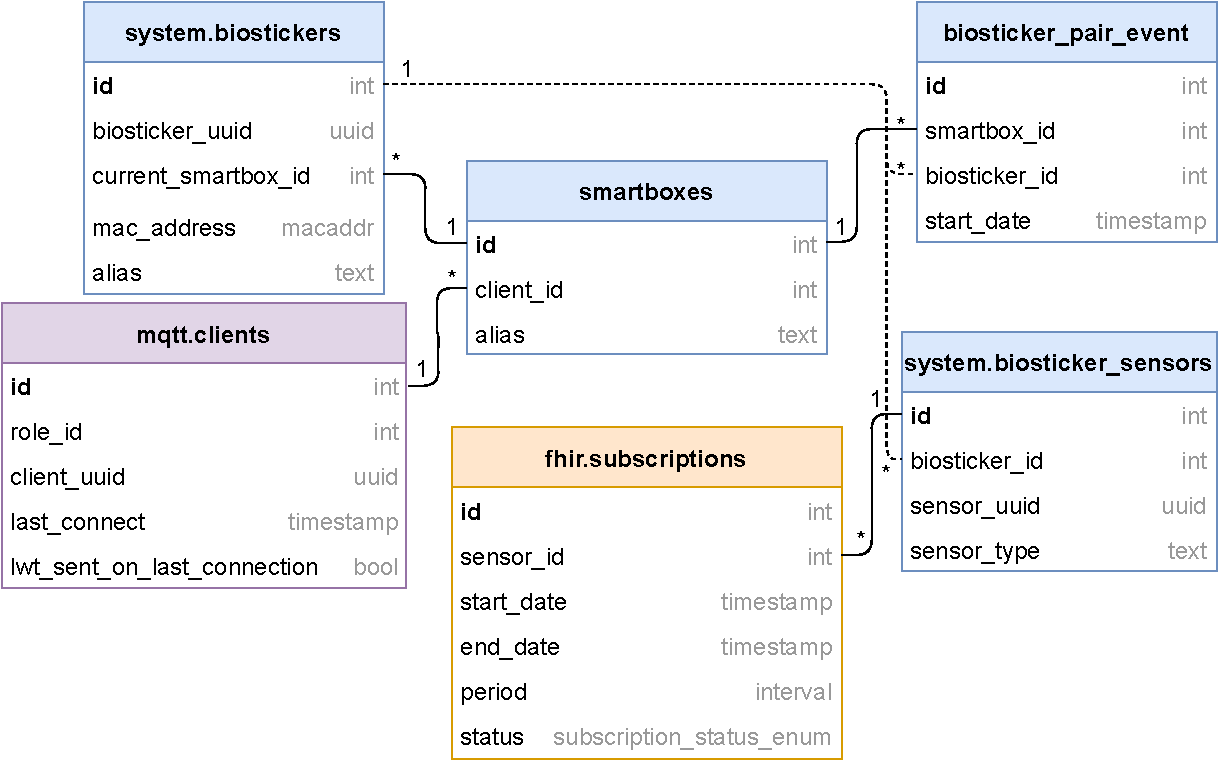
\includegraphics[width=\linewidth]{images/database-schema-fhir.pdf}
    \caption[test]{test}
    \label{fig:wow-dbschema-fhir}
\end{figure}
 

\subsubsection{Stored Procedures}

%During development, we noticed that our database service was consuming a concerning amount of resources when 
- de modo a maximizar o desempenho do serviço da base de dados, os diferentes pedidos de base de dados (queries) foram configurados e pré-compilados na base de dados. isto reduz o tamanho dos pedidos enviados à base de dados (pois em vez de enviar transações complexas, executamos apenas uma função na base de dados), faz com que a base de dados não tenha de validar a estrutura dos pedidos (porque já foi pre-compilada), particularmente para eviar injeções de SQL.


Since the \acs{Smart Gateway} makes use of an \acs{RDBMS}, services that access the database use \acf{SQL} to perform requests, such as retrieving data or inserting data. In order to maximize the performance of our data storage solution, we implement ``Stored Procedures'', which are subroutines that are stored in the \acs{RDBMS}. These procedures are pre-compiled \acs{SQL} statements that are defined in the \acs{RDBMS}, 


which improve performance (since the database system no longer needs to validate and compile a complex query)

\section{Connection to the SmartBoxes}

As previously mentioned, the connection to the \textit{SmartBoxes} is performed via \acs{MQTT}. \acs{MQTT} is a centralized protocol, in which the clients (\textit{SmartBoxes}) connect to a broker, which acts as a middle-man for the communication, managing the requests from all clients accordingly. In our system, the broker is contained within the \textit{Smart Gateway}, and is the service responsible for ensuring the communication between the \textit{SmartBoxes} and our \acs{IoT} system.

\paragraph{} To implement this \acs{MQTT} broker, we use the open-source Eclipse Mosquitto\footnote{Eclipse Mosquitto -- An open-source \acs{MQTT} broker: \url{https://mosquitto.org/}}. Mosquitto is a lightweight \acs{MQTT} broker that supports the \acs{MQTT} protocol versions 5.0, 3.1.1 and 3.1 and is widely used by the community, making it a fitting solution for the \acs{WoW} project.

\paragraph{} One of the 



It is extremely flexible since it allows developers to extend its functionality using plugins

exposes an \acs{API}

extensible 

\paragraph{} 


\subsection{Specification for \acs{MQTT} Communication}
- indicar que foi proposta uma especificação para a comunicação MQTT

\subsection{Authorization and Authentication Plugin}
- 
- a segurança no MQTT é feita através de 2 points
- a segurança no mosquitto atualmente é feita através de um ficheiro estático (lol) que define as permissões dos clientes que acedem o servidor.
- de modo a assegurar 

\section{Integration with GlobalCare}

- Mini introdução ao FHIR;
- mencionar camada de interoperabilidade da globalcare;
- indicar que optou-se usar HAPI devido ao facto de ser uma iniciativa open-source suportada por uma empresa de software hospitalar de renome.
- HAPI FHIR é baseada em Java servlets, fazer mini introdução do que são servlets e explicar o porquê de usar Jetty para correr servlets (é um web container, cujo objetivo é correr servlets). 

\subsection{FHIR Server}

- Falar do que são os FHIR Resources, e mais especificamente dos Resources usados para transmitir os dados -> Bundle, Device, Observation
- Apresentação do diagrama de comunicação de informação

\section{Summary}

In this chapter, we presented the different components which form the \textit{Smart Gateway}. In the chapter, we evaluate the performance of our proposed solution through a hospital trial.